\chapter{Estado del arte: Redes de sensores}

En el estudio de los distintos sistemas domoticos vemos que estos realmente solo son una red de sensores y actuadores
con un enfoque muy concreto, la vivienda. Por ello veamos con mas detenimiento las redes de sensores, en especial las
redes inal\'ambricas.

La idea de una red de sensores surge gracias a las posibilidades que nos da la tecnolog\'ia de crear una red de
dispositivos de captura constante, que nos permita registrar y almacenar una determinada informaci\'on, transmitir datos
de un dispositivo a otro, y despu\'es retransmitir toda la informaci\'on para almacenarla en una localizaci\'on central.

Las redes de sensores con cable no son nuevas y sus funciones han sido, tradicionalmente, medir niveles de temperatura,
l\'iquido, humedad etc. La diferencia entre estos sensores que todos conocemos y la nueva generaci\'on de WSN es que estos
\'ultimos son inteligentes, capaces de poner en marcha una acci\'on seg\'un la informaci\'on que vayan acumulando y, adem\'as, no
est\'an limitados por su conexi\'on a trav\'es de un cable e incluso puede ser m\'oviles. 

Los nuevos avances en la fabricaci\'on de microchips, los nuevos est\'andares de comunicaciones inal\'ambricas, las nuevas
funcionalidades de routers y equipamientos de red, los nuevos desarrollos de software y programas inform\'aticos est\'an
logrando eliminar los cables de las redes de sensores, multiplicando as\'i su potencial.

\section{Redes inal\'ambricas de sensores} 

Una red de sensores (o WSN, Wireless Sensor Network, en ingl\'es) es una red de dispositivos, equipados con sensores, y de
comunicaci\'on inal\'ambrica que permiten formar redes ad-hoc sin infraestructura f\'isica preestablecida ni administraci\'on
central.


La expresi\'on ad-hoc hace referencia a una red en la que no hay un nodo central, sino que todos los dispositivos est\'an en
igualdad de condiciones. Ad-hoc es el modo m\'as sencillo para crear una red, un tipo de red formada por un grupo de
nodos que forman una red temporal sin la ayuda de ninguna infraestructura externa. Para que esto se pueda llevar a la
pr\'actica es necesario que los nodos se puedan ayudar mutuamente para conseguir un objetivo com\'un: que cualquier paquete
llegue a su destino aunque el destinatario no sea accesible directamente desde el origen.


El protocolo de encaminamiento es el responsable de descubrir las rutas entre los nodos para hacer posible la
comunicaci\'on. Las redes de sensores son un concepto relativamente nuevo en adquisici\'on y tratamiento de datos con
m\'ultiples aplicaciones en distintos campos, tales como entornos industriales, dom\'otica, entornos militares, detecci\'on
ambiental. Esta clase de redes se caracterizan por su facilidad de despliegue y por ser autoconfigurables, pudiendo
convertirse en todo momento en emisor, receptor, ofrecer servicios de encaminamiento entre nodos sin visi\'on directa,
as\'i como registrar datos referentes a los sensores locales de cada nodo.


Las redes de sensores es un tema muy activo de investigaci\'on en varias universidades, aunque ya empiezan a existir
aplicaciones comerciales basadas en este tipo de redes. 


La lista de aplicaciones donde las WSN encuentran utilidad puede ser ingente y abierta a la creatividad. Los usos m\'as
t\'ipicos est\'an relacionados con tareas de supervisi\'on, seguimiento y control. 



Algunos de los usos espec\'ificos son:

\begin{itemize}
\item Dom\'otica.
\item Control/Supervisi\'on del medio ambiente.
\item Detecci\'on ac\'ustica.
\item Detecci\'on s\'ismica.
\item Detecci\'on/Control actividad nuclear.
\item Vigilancia militar.
\item Seguimiento de inventario.
\item Seguimiento de objetos, personas.
\item Supervisi\'on m\'edica.
\item Espacios inteligentes.
\item Control de procesos operativos.
\item Gesti\'on tr\'afico en ciudades y carreteras.
\end{itemize}

 

\section{Arquitectura del sistema}

Las redes de sensores est\'an formadas por un conjunto de peque\~nos dispositivos con capacidad limitada de c\'omputo y
comunicaci\'on, cuyo tiempo de vida depende de una bater\'ia adjunta al dispositivo. El tiempo de vida de la red de
sensores depender\'a por tanto del tiempo de vida de la bater\'ia de sus nodos.

Estos dispositivos se encuentran dispersos de manera ad-hoc en una determinada \'area a monitorizar. En redes de
comunicaci\'on, dicha expresi\'on hace referencia a una red en la que no hay un nodo central, sino que todos los nodos
est\'an en igualdad de condiciones.

T\'ipicamente, el modelo seguido por las aplicaciones es el siguiente: realizar una serie de mediciones sobre el medio,
transformar dicha informaci\'on en digital en el propio nodo y transmitirla fuera de la red de sensores v\'ia un elemento
gateway a una estaci\'on base, donde la informaci\'on pueda ser almacenada y tratada temporalmente para acabar finalmente
en un servidor con mayor capacidad que permita componer un hist\'orico o realizar an\'alisis de datos, por lo tanto,
podemos encontrarnos: 

\begin{itemize}
\item nodos inal\'ambricos 
\item puertas de enlace 
\item estaciones base
\end{itemize}

\begin{figure}[htbp]
	\centering
		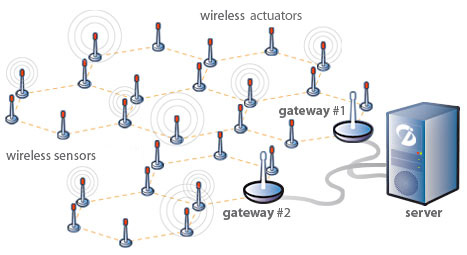
\includegraphics[width=0.8\textwidth]{imagenes/red_de_sensores.jpg}
	\caption{Red de sensores}
	\label{fig:red_de_sensores}
\end{figure}

 

\subsection{Nodo inal\'ambrico}
Los nodos inal\'ambrico son dispositivos electr\'onicos capaces de captar informaci\'on proveniente del entorno en el que se
encuentran, procesarla y transmitirla inal\'ambricamente hacia otro destinatario. 

El tama\~no de un nodo puede variar desde una caja de zapatos hasta un grano de polvo. El coste de estos nodos es
igualmente variable, extendi\'endose desde centenas de euros a algunos c\'entimos, dependiendo del tama\~no de la red del
sensor y de la complejidad requerida de cada nodo individual. Las limitaciones de tama\~no y de coste en el nodo del
sensor dan lugar a restricciones en recursos tales como energ\'ia, memoria, velocidad de proceso y anchura de banda.

El hardware de cada uno de estos dispositivos tiene varias partes bien diferenciadas como se puede ver en la figura \ref{fig:partes_nodo}.

\begin{figure}[htbp]
	\centering
		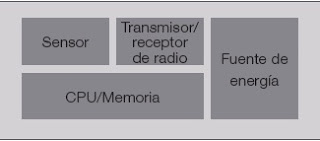
\includegraphics{imagenes/partes_nodo.jpg}
	\caption{Partes de un nodo}
	\label{fig:partes_nodo}
\end{figure}

 


\subsubsection{Procesador}
Es el componente que interpreta y procesa los datos para transmitirlos a otra estaci\'on. Tambi\'en gestiona el
almacenamiento de datos en la memoria. Puesto que de un nodo sensor se espera una comunicaci\'on y una recogida de datos
mediante sensores, debe existir una unidad de procesado, que se encargue de gestionar todas estas operaciones. 

Hay muchos tipos diferentes de productos disponibles en el mercado para ser integrados en un nodo, como
microcontroladores, microprocesadores y FPGA. 

\begin{description}
	\item[FPGA]
	Actualmente \'estas presentan varias desventajas, la mayor de ellas es el consumo. A pesar de que en el mercado
podemos encontrar FPGAs de bajo consumo, este consumo no es lo suficientemente bajo como deber\'ia ser para este tipo de
nodos. Esto no significa que en un futuro cercano, \'estas sean una buena opci\'on si se consigue que reduzcan el consumo.
	\item[Microprocesadores]
	Han sido sustituidos por los microcontroladores, ya que \'estos integran dentro de un mismo
dispositivo, un microprocesador y memoria.
	\item[Microcontroladores]
	Como se ha dicho, incluyen un microprocesador y memoria, pero adem\'as tienen una interface para
ADCs, UART, SPI, temporizadores y contadores. Hay muchos tipos de microcontroladores que van desde los 4 bits hasta 64
bits, con una variaci\'on del numero de temporizadores, con diferentes consumos de energ\'ia, etc...
\end{description}
 

Algunos de los m\'as utilizados son los siguientes procesadores de bajo consumo:

\begin{itemize}
\item ARM7
\item Atmel AVR
\item Intel Xscale
\item PIC
\end{itemize}


\subsubsection{Alimentaci\'on}
Normalmente la fuente de alimentaci\'on son bater\'ias dif\'icilmente sustituibles o transformadores con salida adecuada para
el nodo si se dispone de toma de corriente. Para las situaciones en donde no se dispone de red el\'ectrica y las
posibilidad de sustituir las bater\'ias es muy complicada, se est\'an estudiando diferentes t\'ecnicas para alimentar el
sensor, como puede ser mediante placas solares. 

Ante la limitaci\'on de la vida \'util del dispositivo hay que realizar una gesti\'on eficiente del consumo energ\'etico. El
consumo de energ\'ia viene dado por lo que consumen los sensores, la comunicaci\'on y el procesado. La mayor cantidad de
energ\'ia es consumida en la transmisi\'on de informaci\'on, siendo menor en el procesado y uso de los sensores.

\ Las bater\'ias son la principal fuente de energ\'ia de los nodos, pudiendo ser recargables o no recargables. Actualmente
se est\'an estudiando sistemas basados en energ\'ia renovables para solucionar el problema de la energ\'ia en estos nodos,
basados en energ\'ia solar, termo generaci\'on, energ\'ia basada en vibraciones, etc...

\subsubsection{Comunicaci\'on Inal\'ambrica }
El dispositivo de comunicaci\'on se trata de un dispositivo v\'ia radio que permite enviar y recibir datos para comunicarse
con otros dispositivos dentro de su rango de transmisi\'on. 

Los nodos usan la banda ISM que son bandas reservadas internacionalmente para uso no comercial de radiofrecuencia
electromagn\'etica en \'areas industrial, cient\'ifica y m\'edica. El uso de estas bandas de frecuencia est\'a abierto a todo el
mundo sin necesidad de licencia, respetando las regulaciones que limitan los niveles de potencia transmitida. Los
medios a elegir para realizar una comunicaci\'on inal\'ambrica son varios, radio frecuencia, comunicaci\'on \'optica mediante
l\'aser e infrarrojos. 

La comunicaci\'on por l\'aser es la que menos energ\'ia consume pero requiere de una comunicaci\'on visual entre emisor y
receptor, y adem\'as tambi\'en depende de las condiciones atmosf\'ericas. 

Los infrarrojos como el l\'aser, no necesitan antena, aunque es bastante limitado en su capacidad de transmisi\'on. 

La radio frecuencia, RF, es la m\'as adecuada para usar en aplicaciones inal\'ambricas. Las WSN usan las frecuencias de
comunicaci\'on que andan entre 433 MHz y 2.4 Ghz.

\subsubsection{Sensores}
Los sensores son dispositivos hardware que producen una respuesta medible ante un cambio en un estado f\'isico, como puede
ser temperatura o presi\'on. Los sensores detectan o miden cambios f\'isicos en el \'area que est\'an monitorizando. La se\~nal
anal\'ogica continua detectada es digitalizada por un convertidor anal\'ogico digital y enviada a un controlador para ser
procesada.

Las caracter\'isticas y requerimientos que un sensor debe tener son un peque\~no tama\~no, un consumo bajo de energ\'ia, operar
en densidades volum\'etricas altas, ser aut\'onomo y funcionar desatendidamente y tener capacidad para adaptarse al
ambiente. 

Los sensores pueden estar clasificados en tres categor\'ias: 

\begin{description}
\item [Sensores pasivos omnidireccionales]
 Los sensores pasivos captan los datos sin necesidad de manipular el entorno.
Son autoalimentados y solo usan la energ\'ia para amplificar la se\~nal anal\'ogica captada. No hay ninguna noci\'on de direcci\'on involucrada en estas mediciones.

\item [Sensores pasivos unidireccionales] 
Son sensores pasivos que tienen bien definida la direcci\'on desde donde deben
captar la informaci\'on. Un ejemplo t\'ipico es una c\'amara. 

\item [Sensores activos] Este tipo de sensores sondean el ambiente, por ejemplo un radar o un sonar o alg\'un tipo de
sensor s\'ismico que generan ondas expansivas a trav\'es de peque\~nas explosiones.
\end{description}

\subsubsection{Memoria}
Desde el punto de vista de gasto de energ\'ia, las clases m\'as relevantes de memoria son la memoria integrada en el chip de
un microcontrolador y la memoria flash, la memoria RAM fuera del chip es raramente usada.

Las memorias flash son usadas gracias a su bajo coste y su gran capacidad de almacenamiento. La memoria flash es una
forma desarrollada de la memoria EEPROM que permite que m\'ultiples posiciones de memoria sean escritas o borradas en una
misma operaci\'on de programaci\'on mediante impulsos el\'ectricos, frente a las anteriores que s\'olo permite escribir o
borrar una \'unica celda cada vez. Por ello, flash permite funcionar a velocidades muy superiores cuando los sistemas
emplean lectura y escritura en diferentes puntos de esta memoria al mismo tiempo. Las memorias flash son de car\'acter no
vol\'atil, una caracter\'istica muy valorada para la multitud de usos en los que se emplea este tipo de memoria. 

Los requerimientos de memoria dependen mucho de la capacidad que necesite nuestra aplicaci\'on. Hay dos categor\'ias de
memorias seg\'un el prop\'osito del almacenamiento: 

\begin{itemize}
\item Memoria usada para almacenar los datos recogidos por la aplicaci\'on. 
\item Memoria usada para almacenar el programa del dispositivo.
\end{itemize}


\subsection{Puerta de enlace}
Elementos para la interconexi\'on entre la red de sensores y una red de datos. Es un nodo especial sin elemento sensor,
cuyo objetivo es actuar como puente entre dos redes de diferente tipo. 

En este tipo de aplicaciones donde se usan redes de sensores, \'estas no pueden operar completamente aisladas y deben
contar con alguna forma de monitoreo y acceso a la informaci\'on adquirida por los nodos de la red de sensores. De aqu\'i
surge la necesidad de conectar las redes de sensores a infraestructuras de redes existentes tales como Internet, redes
de \'area local (LAN) e intranets privadas. 

Los dispositivos que realizan la funci\'on de interconectar dos redes de diferente naturaleza se les llama dispositivo
puerta de enlace; pero el t\'ermino m\'as conocido en el ambiente de las redes es gateway. 

\subsection{Estaci\'on base}
Recolector de datos basado en un ordenador com\'un o sistema empotrado. En una estructura normal todos los datos van a
parar a un equipo servidor dentro de una base de datos, desde donde los usuarios pueden acceder remotamente y poder
observar y estudiar los datos.

\section{Topolog\'ias de red} 

Hay varias arquitecturas que pueden ser usadas para implementar una aplicaci\'on de WSN como pueden ser estrella, malla o
una h\'ibrida entre ellas dos. Cada topolog\'ia presenta desaf\'ios, ventajas y desventajas. Para entender las diferentes
topolog\'ias es necesario conocer los diferentes componentes de la WSN. 

\begin{description}
\item [Nodos finales] Compuesto por sensores y actuadores donde se capturan los datos sensores. 

\item [Routers] Dan cobertura a redes muy extensas pudiendo salvar obst\'aculos, problemas de congesti\'on en la emisi\'on de
la informaci\'on y posibles fallos en alguno de los aparatos. 

\item [Puertas de enlace] Recoge los datos de la red, sirve como punto de uni\'on con una red LAN o con Internet. 
\end{description}

Cada topolog\'ia es apropiada bajo ciertas circunstancias y ser inapropiada en otras. 

\subsection{Topolog\'ia en estrella}
Una topolog\'ia en estrella es un sistema donde la informaci\'on enviada s\'olo da un salto y donde todos los nodos sensores
est\'an en comunicaci\'on directa con la puerta de enlace.

Todos los nodos sensores son id\'enticos, nodos finales, y la puerta de enlace capta la informaci\'on de todos ellos. La
puerta de enlace tambi\'en es usada para transmitir datos al exterior y permitir la monitorizaci\'on de la red. 

Los nodos finales no intercambian informaci\'on entre ellos, sino que usan la puerta de enlace para ello, si es necesario.

\begin{figure}[htb]
    \centering
    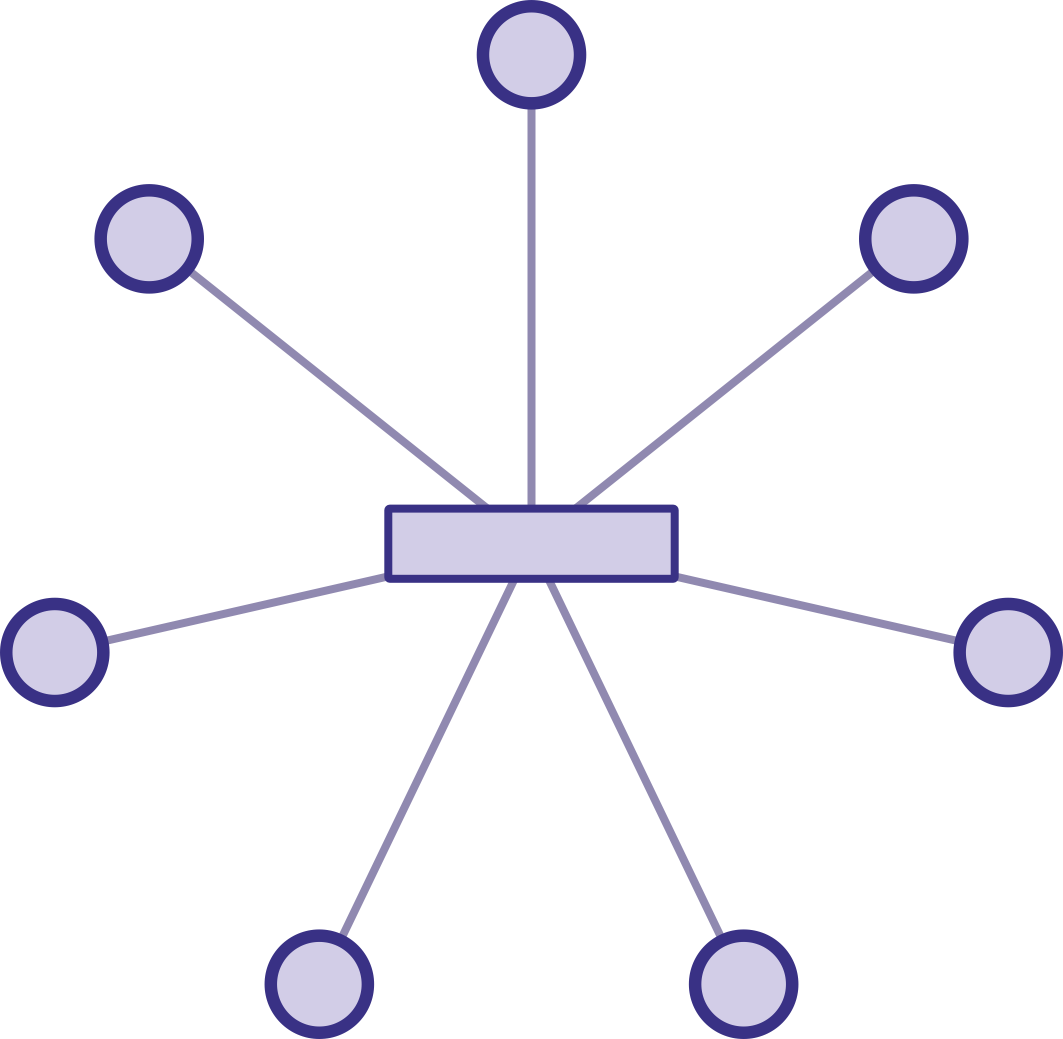
\includegraphics[width=0.4\textwidth]{imagenes/estrella.png}
    \caption{Topología en estrella}
    \label{fig:top_estrella}
\end{figure}

La topolog\'ia en estrella es la que menor gasto de energ\'ia desarrolla, pero por el contrario esta limitada por la
distancia de transmisi\'on v\'ia radio entre cada nodo y la puerta de enlace. Tampoco tiene un camino de comunicaci\'on
alternativo en caso de que uno de los nodos tenga obstruido el camino de comunicaci\'on, lo que lleva a que en este caso
la informaci\'on de ese nodo sea perdida.


\subsection{Topolog\'ia en malla}
La topolog\'ia en malla es un sistema multisalto, donde todos los nodos son routers y son id\'enticos. Cada nodo puede
enviar y recibir informaci\'on de otro nodo y de la puerta de enlace. A diferencia de la topolog\'ia en estrella, donde los
nodos solo pueden hablar con la puerta de enlace, en \'esta los nodos pueden enviarse mensajes entre ellos. 

\begin{figure}[htb]
    \centering
    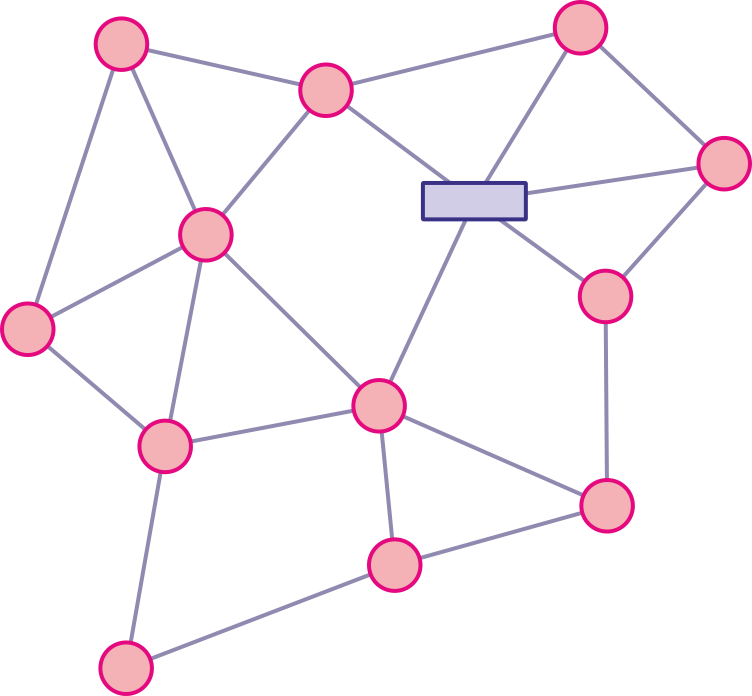
\includegraphics[width=0.6\textwidth]{imagenes/malla.png}
    \caption{Topología en malla}
    \label{fig:top_malla}
\end{figure}

La propagaci\'on de los datos a trav\'es de los nodos hacia la puerta de enlace hace posible, por lo menos en teor\'ia, crear
una red con una extensi\'on posible ilimitada. Este tipo, tambi\'en es altamente tolerante a fallos ya que cada nodo tiene
diferentes caminos para comunicarse con la puerta de enlace. Si un nodo falla, la red se reconfigurar\'a alrededor del
nodo fallido autom\'aticamente. Dependiendo del n\'umero de nodos y de la distancia entre ellos, la red puede experimentar
periodos de espera elevados a la hora de mandar la informaci\'on. 

\subsection{Topolog\'ia h\'ibrida (estrella-malla)}
Este tipo de red busca combinar las ventajas de los otros dos tipos, la simplicidad y el bajo consumo de una topolog\'ia en estrella, as\'i como la posibilidad de cubrir una gran extensi\'on y de reorganizarse ante fallos de la topolog\'ia en malla.

\begin{figure}[htb]
    \centering
    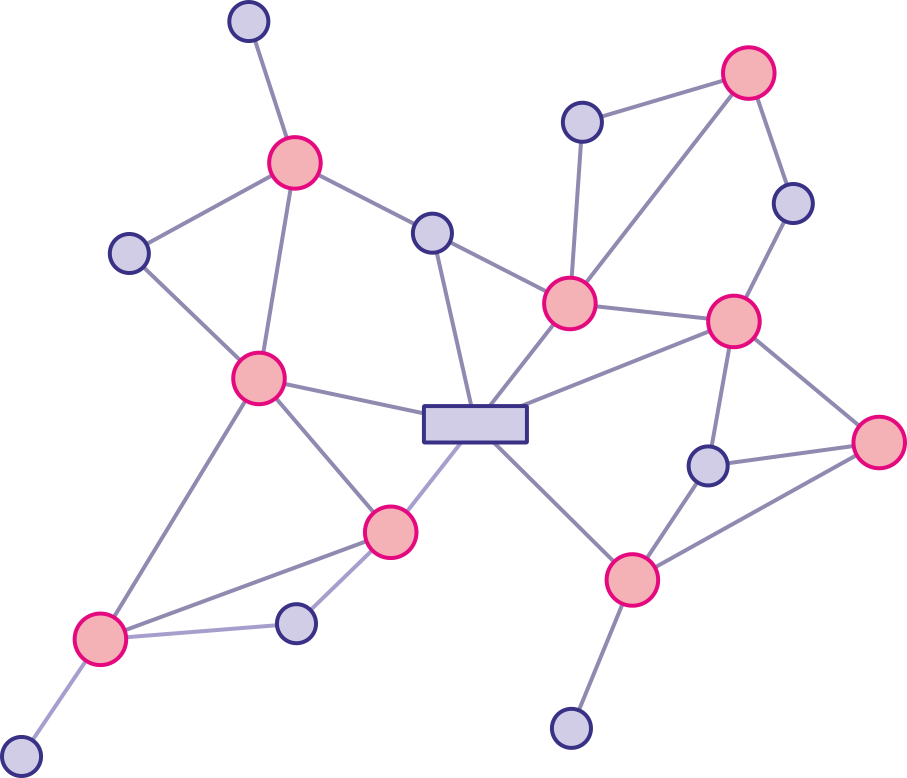
\includegraphics[width=0.7\textwidth]{imagenes/hibridamalla.png}
    \caption{Topología híbrida}
    \label{fig:top_hibrida}
\end{figure}

 Este tipo crea una red en estrella alrededor de routers pertenecientes a una red en malla. Los routers dan la
posibilidad de ampliar la red y de corregir fallos en estos nodos y los nodos finales se conectan con los routers
cercanos ahorrando energ\'ia.

\section {Redes ad-hoc y tecnolog\'ia inal\'ambrica} 

Las redes mas usadas en las implantaciones de redes de sensores inal\'ambricas son las redes malladas tipo ad-hoc. Son
redes sin infraestructura, flexibles en las cuales todas las estaciones ofrecen servicios de encaminamiento para
permitir la comunicaci\'on de estaciones que no tienen conexi\'on inal\'ambrica directa.

La principal caracter\'istica de las redes m\'oviles ad-hoc es que todos los dispositivos que forman parte de la red, adem\'as
de funcionar como terminales finales, realizan tambi\'en funciones de retransmisi\'on de paquetes t\'ipicamente asociadas a
routers. Esta cualidad nos permite encaminar paquetes a destinos sin cobertura directa a trav\'es de otros nodos
intermedios que se encuentren en la red. De este modo se nos ofrece la posibilidad de incrementar de una manera
extraordinaria la movilidad y el tama\~no de una red de datos inal\'ambrica. 

La funcionalidad principal de estas redes es la de crear de una manera r\'apida y eficaz una red temporal en lugares
carentes de una infraestructura de red. Las principales caracter\'isticas de una red ad-hoc son: 

\begin{description}

\item[Movilidad]
Este aspecto es la raz\'on de ser de las redes ad-hoc. Los nodos se pueden reposicionar o simplemente ser
m\'oviles, siempre que no salgan del alcance radio. Se pueden desplegar r\'apidamente sin la necesidad de descubrir la zona
o formar grupos, es decir, cada nodo es individual y solvente. 

\item[Multisalto (Multihopping)]
Una red multihopping es una red donde el camino de la fuente al destino atraviesa
varios nodos intermedios. 

\item[Autoorganizaci\'on]
La red de forma aut\'onoma debe determinar sus propios par\'ametros de configuraci\'on: direcci\'on,
encaminamiento, clustering, indicador de posici\'on, etc. 

\item[Conservaci\'on de la energ\'ia] 
Los nodos m\'oviles, tienen una bater\'ia limitada y a no ser que dispongan de alg\'un
mecanismo de carga (por ejemplo, un panel solar), no tienen capacidad de recarga. Es muy importante dise\~nar unos
protocolos (MAC, encaminamiento) eficientes, con la finalidad de mejorar el rendimiento y prolongar la autonom\'ia de las
bater\'ias. 

\item[Escalabilidad]
En algunos tipos de redes, el n\'umero de nodos puede crecer hasta llegar a varios miles. Como no
existe un access point concreto, la incorporaci\'on y descarte de nodos es un proceso sencillo y transparente. 

\item[Seguridad]
Las redes inal\'ambricas son vulnerables a ataques, y las redes ad-hoc lo son especialmente. Pueden
padecer tanto ataques activos como pasivos y el atacante puede emular a un nodo leg\'itimo y capturar paquetes de datos y
control, destruir tablas de encaminamiento, etc.
\end{description}

\subsection{Protocolos}
Sin embargo, para que lo anterior sea viable se hace necesaria la inclusi\'on en la red de protocolos de encaminamiento
que nos permitan crear las rutas hacia los destinos deseados. 

Los protocolos tradicionales propios de redes fijas no se adaptan bien a este tipo de entornos tan din\'amicos y, por
tanto, ser\'a necesario el dise\~no espec\'ifico de protocolos para proporcionar un comportamiento eficiente a la red. 

La principal clasificaci\'on es la que diferencia entre protocolos proactivos y reactivos (o bajo demanda): 

Los protocolos proactivos, peri\'odicamente se env\'ia informaci\'on de encaminamiento para que en cualquier momento cualquier
nodo pueda comunicarse con cualquier otro de la red. Esta caracter\'istica proporciona una r\'apida respuesta ante
solicitudes de ruta y ofrece un buen comportamiento en situaciones donde la tasa de movilidad es alta. Sin embargo la
sobrecarga que se introduce en la red con informaci\'on de control es alta. Entre estos protocolos podemos destacar el
protocolo DSDV (Destination-Sequenced Distance Vector).

Por otra parte, los protocolos reactivos s\'olo crean rutas cuando es necesario. Son protocolos bajo demanda donde la
sobrecarga es mucho menor, pero los retrasos de establecimiento de rutas son mayores. Podemos nombrar AODV (Ad hoc
On-Demand Distance Vector) como protocolo reactivo. Existen algunos protocolos h\'ibridos en los que se mantiene una
filosof\'ia proactiva en un \'ambito local y reactiva a nivel m\'as global, como el protocolo ZRP (Zone Routing Protocol).

Los principales protocolos utilizados son:

\begin{description}
\item[Destination-Sequenced Distance Vector (DSDV)] 
DSDV es esencialmente una modificaci\'on del algoritmo de
encaminamiento Vector Distancia Bell-man-Ford, bien conocido por su utilidad en redes fijas, como por ejemplo en el
protocolo RIP. En este algoritmo, los nodos vecinos intercambian peri\'odicamente (proactivo) sus tablas de
encaminamiento enteras para estimar la distancia a la que se encuentran los dem\'as nodos no vecinos. Las modificaciones
introducidas por DSDV proporcionan b\'asicamente la obtenci\'on de rutas sin bucles mediante la introducci\'on de n\'umeros de
secuencia para la determinaci\'on de las rutas m\'as nuevas. Aunque DSDV s\'olo proporciona un camino para cada destino,
siempre elige el camino m\'as corto bas\'andose en el n\'umero de saltos hacia este destino. DSDV utiliza dos tipos de
mensajes de actualizaci\'on, uno m\'as grande (full-dump) y otro mucho m\'as peque\~no (incremental). Los mensajes
incrementales pueden utilizarse para actualizaciones intermedias entre env\'ios peri\'odicos (full-dump) de la tabla entera
de encaminamiento. Adem\'as se realizan estimaciones de los tiempos de establecimientos de ruta que retrasar\'an el env\'io
de mensajes incrementales para evitar env\'ios en cadena de estos mensajes. 

\item[Optimized Link-State Routing Algorithm (OLSR)]
OLSR incorpora la filosof\'ia utilizada en protocolos tradicionales
como OSPF de Estado de los Enlaces. En este algoritmo todos los nodos se intercambian mensajes para formarse
una visi\'on consistente de toda la red y as\'i poder decidir el encaminamiento de paquetes. OLSR adolece del mismo
problema que DSDV debido a la necesidad de intercambio de un gran n\'umero de mensajes peri\'odicos (proactivo). Aqu\'i, el
problema podr\'ia llegar a ser mayor, ya que adem\'as de mensajes [91?]hello[92?] a los vecinos, env\'ia mensajes de control
[91?]tc[92?] (Topology Control) que se retransmiten a todos los nodos de la red. Sin embargo se ha conseguido una gran
optimizaci\'on en la retransmisi\'on de estos mensajes con la incorporaci\'on de la t\'ecnica de retransmisi\'on multipunto, a
trav\'es de la cual, los mensajes s\'olo son retransmitidos por el m\'inimo n\'umero de nodos necesarios para alcanzar a todos
los dem\'as. Estos nodos son conocidos como grupo de retransmisores multipunto (MPR's). 

\item[Dynamic Source Routing (DSR)]
El protocolo DSR se fundamenta en el encaminamiento desde el origen, es decir, los
paquetes de datos incluyen una cabecera de informaci\'on acerca de los nodos exactos que deben atravesar. No requiere
ning\'un tipo de mensajes peri\'odicos (reactivo), disminuyendo as\'i la sobrecarga con mensajes de control. Adem\'as ofrece la
posibilidad de obtener, con la solicitud de una ruta, m\'ultiples caminos posibles hacia el destino. Tampoco son un
problema, a diferencia de la mayor\'ia de protocolos de encaminamiento en este tipo de redes, los enlaces
unidireccionales. Para poder realizar el encaminamiento en el origen, a cada paquete de datos se le inserta una
cabecera DSR de opciones que se colocar\'a entre la cabecera de transporte y la IP. Entre dichas opciones se incluir\'a la
ruta que debe seguir el paquete nodo a nodo. Cada nodo mantiene una memoria cach\'e de rutas en la que se van almacenando
las rutas obtenidas a trav\'es de procesos de descubrimiento de rutas ya sean propias o obtenidas a trav\'es de escuchas en
la red. En los procesos de descubrimiento de rutas se generan mensajes de solicitud, respuesta y error siendo estos
mensajes route request, reply y error respectivamente. 

\item[Ad Hoc On-Demand Distance Vector (AODV)]
En el protocolo AODV los nodos mantienen una tabla de encaminamiento para
los destinos conocidos (empleando el algoritmo vector distancia). Inicialmente esta tabla estar\'a formada por sus
vecinos. Solamente se le a\~nadir\'an destinos nuevos cuando sea necesario, es decir, cuando un nodo necesita comunicarse
con otro que no est\'a en su tabla, inicia un proceso de descubrimiento de ruta (reactivo) hacia el destino concreto.
Para ello se emiten mensajes de descubrimiento de ruta rreq que se van propagando entre todos los nodos de
modo similar al DSR. En cambio, aqu\'i los nodos generan una tabla de encaminamiento inversa para que puedan regresar las
contestaciones rrep a las solicitudes de ruta al nodo que la origin\'o. Se recomienda el uso de mensajes
hello entre vecinos para determinar la conectividad, aunque para reducir el volumen de estos mensajes, s\'olo
debe permitirse su env\'io a los nodos que est\'en transmitiendo datos. Debemos destacar adem\'as la utilizaci\'on de las
t\'ecnicas de <<b\'usqueda secuencial por anillos>> y <<reparaci\'on local del
enlace>> as\'i como tambi\'en que es capaz de proporcionar soporte multicast.
\end{description}

\subsection{Tecnolog\'ia inal\'ambrica}
Las tecnolog\'ias inal\'ambricas pueden clasificarse en cinco grandes grupos, de acuerdo con la distancia que viaja cada
tipo de se\~nal.

Primero est\'an las comunicaciones satelitales, como el sistema de posicionamiento global (GPS, por sus siglas en ingl\'es),
formado por 24 sat\'elites, los cuales env\'ian constantemente se\~nales a dispositivos en tierra. Sin embargo, estas se\~nales
s\'olo viajan del sat\'elite al aparato receptor.

Otra categor\'ia, y con se\~nales de dos v\'ias, est\'an las tecnolog\'ias de telefon\'ia movil de cobertura amplia como GSM y CDMA.
Entre las versiones avanzadas de tercera generaci\'on (3G) destacan HSDPA y LTE.

Una tercera categor\'ia incluye se\~nales de menor alcance utilizadas para conectar dispositivos dentro de una habitaci\'on o
un edificio, como los sistemas Wi-Fi para conectarse a Internet dentro de hoteles o aeropuertos, o Zigbee, protocolo de
comunicaciones inal\'ambricas que sirve para interconectar sensores.

En cuarto lugar est\'an los protocolos para enlazar dispositivos en una <<red de \'area personal>>
(PAN, personal area network). Por ejemplo Bluetooth, utilizado para enviar la se\~nal de un tel\'efono movil a un auricular
inal\'ambrico. 

El \'ultimo tipo de comunicaciones son las que se dan cerca de una antena transmisora (NFC, near-field communications). En
este caso, el dispositivo receptor debe estar cerca del sistema emisor, por ejemplo, al pasar por un edificio o en el
transporte p\'ublico.

Estos sistemas de radio son tan diferentes entre s\'i como la luz lo es del sonido. Podemos ver como se distribuyen las
diferentes tecnolog\'ias inal\'ambricas dependiendo de la velocidad de transmisi\'on y de su utilizaci\'on.


 

IMAGEN DE LAS DISTINTAS TECNOLOG\'iAS


 

Claramente se ve que los protocolos m\'as adecuados para ser usados en WSN son los protocolos Bluetooth y Zigbee. A pesar
de que ZigBee es muy similar a Bluetooth podemos encontrar algunas diferencias que hacen m\'as adecuado el protocolo
Zigbee para las WSN: 

\begin{itemize}
\item Una red ZigBee puede constar de un m\'aximo de 65535 nodos distribuidos en subredes de 255 nodos, frente a los 8
m\'aximos de una subred Bluetooth. 
\item Zigbee tiene un menor consumo el\'ectrico que el Bluetooth. Este menor consumo se debe a que el sistema ZigBee se
queda la mayor parte del tiempo dormido, mientras que en una comunicaci\'on Bluetooth esto no se puede dar, y siempre se
est\'a transmitiendo y/o recibiendo.
\end{itemize}



\subsection{Zigbee}
ZigBee es el nombre de la especificaci\'on de un conjunto de protocolos de alto nivel de comunicaci\'on inal\'ambrica para su
utilizaci\'on con radiodifusi\'on digital de bajo consumo, basada en el est\'andar IEEE 802.15.4 de redes inal\'ambricas de
\'area personal (wireless personal area network, WPAN).

Su objetivo son las aplicaciones que requieren comunicaciones seguras con baja tasa de env\'io de datos y maximizaci\'on de
la vida \'util de sus bater\'ias.

En principio, el \'ambito donde se prev\'e que esta tecnolog\'ia cobre m\'as fuerza es en dom\'otica, como puede verse en los
documentos de la ZigBee Alliance, la raz\'on de ello son diversas caracter\'isticas que lo diferencian de otras
tecnolog\'ias:

\begin{itemize}
\item Su bajo consumo.
\item Su topolog\'ia de red en malla.
\item Su f\'acil integraci\'on (se pueden fabricar nodos con muy poca electr\'onica).
\end{itemize}
ZigBee utiliza la banda ISM para usos industriales, cient\'ificos y m\'edicos; en concreto, 868 MHz en Europa, 915 en
Estados Unidos y 2,4 GHz en todo el mundo. Sin embargo, a la hora de dise\~nar dispositivos, las empresas optar\'an
pr\'acticamente siempre por la banda de 2,4 GHz, por ser libre en todo el mundo.

El desarrollo de la tecnolog\'ia se centra en la sencillez y el bajo costo m\'as que otras redes inal\'ambricas semejantes de
la familia WPAN, como por ejemplo Wi-Fi o Bluetooth. El nodo ZigBee m\'as completo requiere en teor\'ia cerca del 10\% del
hardware de un nodo Bluetooth o Wi-Fi t\'ipico.

\subsubsection{Tipos de dispositivos}
Se definen tres tipos distintos de dispositivo ZigBee seg\'un su papel en la red:

\begin{itemize}
\item Coordinador ZigBee (ZigBee Coordinator, ZC): el tipo de dispositivo m\'as completo. Debe existir al menos uno por
red. Sus funciones son las de encargarse de controlar la red y los caminos que deben seguir los dispositivos para
conectarse entre ellos.
\item Router ZigBee (ZigBee Router, ZR): interconecta dispositivos separados en la topolog\'ia de la red, adem\'as de
ofrecer un nivel de aplicaci\'on para la ejecuci\'on de c\'odigo de usuario.
\item Dispositivo final (ZigBee End Device, ZED): posee la funcionalidad necesaria para comunicarse con su nodo padre
(el coordinador o un router), pero no puede transmitir informaci\'on destinada a otros dispositivos. De esta forma, este
tipo de nodo puede estar dormido la mayor parte del tiempo, aumentando la vida media de sus bater\'ias. Un ZED tiene
requerimientos m\'inimos de memoria y es por tanto significativamente m\'as barato.
\end{itemize}
Como ejemplo de aplicaci\'on en Dom\'otica, en una habitaci\'on de la casa tendr\'iamos diversos Dispositivos Finales (como un
interruptor y una l\'ampara) y una red de interconexi\'on realizada con Routers ZigBee y gobernada por el Coordinador.

Bas\'andose en su funcionalidad, puede plantearse una segunda clasificaci\'on:

\begin{itemize}
\item Dispositivo de funcionalidad completa (FFD): Tambi\'en conocidos como nodo activo. Es capaz de recibir mensajes en
formato 802.15.4. Gracias a la memoria adicional y a la capacidad de computar, puede funcionar como Coordinador o
Router ZigBee, o puede ser usado en dispositivos de red que act\'uen de interfaz con los usuarios.
\item Dispositivo de funcionalidad reducida (RFD): Tambi\'en conocido como nodo pasivo. Tiene capacidad y funcionalidad
limitadas (especificada en el est\'andar) con el objetivo de conseguir un bajo coste y una gran simplicidad. B\'asicamente,
son los sensores/actuadores de la red.
\end{itemize}



\subsubsection{Estrategias de conexi\'on de los dispositivos}
Las redes ZigBee han sido dise\~nadas para conservar la potencia en los nodos <<esclavos>>. De esta forma se consigue el
bajo consumo de potencia. La estrategia consiste en que, durante mucho tiempo, un dispositivo
<<esclavo>> est\'a en modo <<dormido>>, de tal forma que solo se
<<despierta>> por una fracci\'on de segundo para confirmar que est\'a
<<vivo>> en la red de dispositivos de la que forma parte. Esta transici\'on del modo
<<dormido>> al modo <<despierto>> (modo en el que realmente
transmite), dura unos 15ms, y la enumeraci\'on de <<esclavos>> dura alrededor de 30ms, como ya
se ha comentado anteriormente.1

En las redes Zigbee, se pueden usar dos tipos de entornos o sistemas:

\begin{itemize}
\item Con balizas: es un mecanismo de control del consumo de potencia en la red. Permite a todos los dispositivos saber
cu\'ando pueden transmitir. En este modelo, los dos caminos de la red tienen un distribuidor que se encarga de controlar
el canal y dirigir las transmisiones. Las balizas que dan nombre a este tipo de entorno, se usan para poder sincronizar
todos los dispositivos que conforman la red, identificando la red dom\'otica, y describiendo la estructura de la
<<supertrama>>. Los intervalos de las balizas son asignados por el coordinador de red y
pueden variar desde los 15ms hasta los 4 minutos.Este modo es m\'as recomendable cuando el coordinador de red trabaja con
una bater\'ia. Los dispositivos que conforman la red, escuchan a dicho coordinador durante el
<<balizamiento>> (env\'io de mensajes a todos los dispositivos -broadcast-, entre 0,015 y 252
segundos). Un dispositivo que quiera intervenir, lo primero que tendr\'a que hacer es registrarse para el coordinador, y
es entonces cuando mira si hay mensajes para \'el. En el caso de que no haya mensajes, este dispositivo vuelve a
<<dormir>>, y se despierta de acuerdo a un horario que ha establecido previamente el
coordinador. En cuanto el coordinador termina el <<balizamiento>>, vuelve a
<<dormirse>>.
\item Sin balizas: se usa el acceso m\'ultiple al sistema Zigbee en una red punto a punto cercano. En este tipo, cada
dispositivo es aut\'onomo, pudiendo iniciar una conversaci\'on, en la cual los otros pueden interferir. A veces, puede
ocurrir que el dispositivo destino puede no o\'ir la petici\'on, o que el canal est\'e ocupado.Este sistema se usa
t\'ipicamente en los sistemas de seguridad, en los cuales sus dispositivos (sensores, detectores de movimiento o de
rotura de cristales), duermen pr\'acticamente todo el tiempo (el 99,999\%). Para que se les tenga en cuenta, estos
elementos se <<despiertan>> de forma regular para anunciar que siguen en la red. Cuando se
produce un evento (en nuestro sistema ser\'a cuando se detecta algo), el sensor <<despierta>>
instant\'aneamente y transmite la alarma correspondiente. Es en ese momento cuando el coordinador de red, recibe el
mensaje enviado por el sensor, y activa la alarma correspondiente. En este caso, el coordinador de red se alimenta de
la red principal durante todo el tiempo.
\end{itemize}

\subsubsection{Comunicaci\'on y descubrimiento de dispositivos}
Seg\'un la informaci\'on disponible, el descubrimiento de dispositivos puede adecuarse utilizando varios m\'etodos distintos.
Si se conoce la direcci\'on de red, se pide la direcci\'on IEEE utilizando unicast. Sino es as\'i, se pide por broadcast, y
la direcci\'on IEEE forma parte de la respuesta. Los dispositivos hoja (end devices) responden con la direcci\'on propia
solicitada, mientras que routers y coordinadores env\'ian tambi\'en las direcciones de todos los dispositivos asociados a
ellos.

Este protocolo extendido permite indagar acerca de dispositivos dentro de una red y sus servicios ofrecidos a nodos
externos a la misma. Los endpoints pueden informar acerca de estos servicios cuando el protocolo de descubrimiento
dirige mensajes a ellos. Tambi\'en pueden utilizarse servicios de emparejamiento oferta-demanda.

Los identificadores de cluster favorecen la asociaci\'on entre entidades complementarias por medio de tablas de
asociaci\'on, mantenidas en los coordinadores ZigBee ya que estas tablas siempre han de estar disponibles en una red (los
coordinadores son, de entre todos los nodos, los que con mayor seguridad dispondr\'an de una alimentaci\'on continua). Los
backups a estas tablas, de ser necesarios para la aplicaci\'on, han de realizarse en niveles superiores.

Por otra parte, el establecimiento de asociaciones necesita que se haya formado un enlace de comunicaci\'on; tras ello, se
decide si adjuntar un nuevo nodo a la red en funci\'on de la aplicaci\'on y las pol\'iticas de seguridad.

Nada m\'as establecerse la asociaci\'on pueden iniciarse las comunicaciones. El direccionamiento directo utiliza la
direcci\'on de radio y el n\'umero de endpoint; el indirecto necesita toda la informaci\'on relevante (direcci\'on, endpoint,
cluster y atributo) y  la env\'ia al coordinador de la red, que mantiene esta informaci\'on por \'el y traduce sus peticiones
de comunicaci\'on. Este direccionamiento indirecto es especialmente \'util para favorecer el uso de dispositivos muy
sencillos y minimizar el almacenamiento interno necesario. 

Adem\'as de estos dos m\'etodos, se puede hacer broadcast a todos los endpoints de un dispositivo, y direccionamiento de
grupos para comunicarse con grupos de endpoints de uno o varios dispositivos distintos.


\subsubsection{Protocolos}
Los protocolos se basan en algoritmos de red para la construcci\'on de redes ad-hoc de baja velocidad. La mayor\'ia de redes
grandes est\'an pensadas para formar un cluster de clusters. Tambi\'en puede estructurarse en forma de malla o como un solo
cluster. Los perfiles actuales de los protocolos soportan redes que utilicen o no facilidades de balizado.

Las redes sin balizas acceden al canal por medio de CSMA/CA. Los routers suelen estar activos todo el tiempo, por lo que
requieren una alimentaci\'on estable en general. Esto, a cambio, permite redes heterog\'eneas en las que algunos
dispositivos pueden estar transmitiendo todo el tiempo, mientras que otros s\'olo transmiten ante la presencia de
est\'imulos externos. El ejemplo t\'ipico es un interruptor inal\'ambrico: un nodo en la l\'ampara puede estar recibiendo
continuamente ya que est\'a conectado a la red; por el contrario, un interruptor a pilas estar\'ia dormido hasta que el
mecanismo se activa. En una red as\'i la l\'ampara ser\'ia un router o coordinador, y el interruptor un dispositivo final.

Si la red utiliza balizas, los routers las generan peri\'odicamente para confirmar su presencia a otros nodos. Los nodos
pueden desactivarse entre las recepciones de balizas reduciendo su ciclo de servicio (duty cycle). Sin embargo, los
periodos largos con ciclos de servicio cortos necesitan que una temporizaci\'on precisa, lo que puede ir en contra del
principio de bajo coste.

En general, los protocolos ZigBee minimizan el tiempo de actividad de la radio para evitar el uso de energ\'ia. En las
redes con balizas los nodos s\'olo necesitan estar despiertos mientras se transmiten las balizas (adem\'as de cuando se les
asigna tiempo para transmitir). Si no hay balizas, el consumo es asim\'etrico repartido en dispositivos permanentemente
activos y otros que s\'olo no est\'an espor\'adicamente.

Las radios utilizan un espectro de dispersi\'on de secuencia directa. Se utiliza BPSK en los dos rangos menores de
frecuencia, as\'i como un QPSK ortogonal que transmite dos bits por s\'imbolo en la banda de 2,4 GHz. Los rangos de
transmisi\'on oscilan entre los 10 y 75 metros, aunque depende bastante del entorno. La potencia de salida de las radios
suele ser de 0 dBm (1 mW).

